\documentclass[tikz,border=6pt]{standalone}
\usepackage{xcolor}
\usetikzlibrary{arrows.meta,positioning}

\definecolor{blockblue}{HTML}{4A90D9}
\definecolor{linegray}{HTML}{333333}

\begin{document}
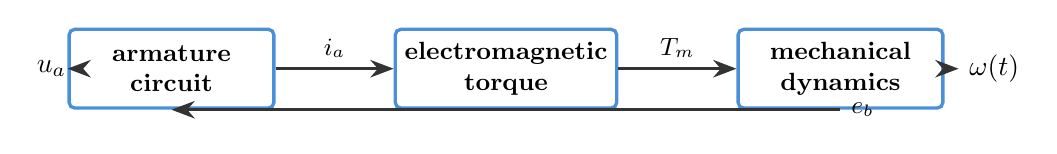
\begin{tikzpicture}[
  >=Stealth,
  line width=1.2pt,
  block/.style={rectangle, draw=blockblue, rounded corners=2pt, minimum width=2.6cm, minimum height=1cm, align=center, font=\small\bfseries},
  flow/.style={->, draw=linegray, line width=1.2pt}
]
  \node[block] (ea) at (0,0) {armature\\circuit};
  \node[block, right=1.5cm of ea] (tm) {electromagnetic\\torque};
  \node[block, right=1.5cm of tm] (me) {mechanical\\dynamics};
  \draw[flow] (-1.2,0) -- (ea) node[left] at (-1.2,0) {$u_a$};
  \draw[flow] (ea) -- node[above, font=\small] {$i_a$} (tm);
  \draw[flow] (tm) -- node[above, font=\small] {$T_m$} (me);
  \draw[flow] (me) -- ++(1.5,0) node[right] {$\omega(t)$};
  \draw[flow] (me.south) |- node[pos=0.25, right, font=\small] {$e_b$} (ea.south);
\end{tikzpicture}
\end{document}
